\documentclass[conference]{IEEEtran}
\IEEEoverridecommandlockouts

\usepackage{cite}
\usepackage{amsmath,amssymb,amsfonts}
\usepackage{algorithmic}
\usepackage{graphicx}
\usepackage{textcomp}
\usepackage{xcolor}
\usepackage{csvsimple}
\usepackage{rotating}
\usepackage{subfig}
\usepackage{float}
\usepackage[toc,page]{appendix}
\usepackage{url}

\usepackage{listings}
\usepackage{color}

\definecolor{dkgreen}{rgb}{0,0.6,0}
\definecolor{gray}{rgb}{0.5,0.5,0.5}
\definecolor{mauve}{rgb}{0.58,0,0.82}

\lstset{frame=tb,
	language=Java,
	aboveskip=3mm,
	belowskip=3mm,
	showstringspaces=false,
	columns=flexible,
	basicstyle={\small\ttfamily},
	numbers=none,
	numberstyle=\tiny\color{gray},
	keywordstyle=\color{blue},
	commentstyle=\color{dkgreen},
	stringstyle=\color{mauve},
	breaklines=true,
	breakatwhitespace=true,
	tabsize=3
}

\usepackage{wrapfig}
\usepackage{lscape}
\usepackage{rotating}
\usepackage{epstopdf}


\def\BibTeX{{\rm B\kern-.05em{\sc i\kern-.025em b}\kern-.08em
		T\kern-.1667em\lower.7ex\hbox{E}\kern-.125em}}
\graphicspath{ {fig/} }

\begin{document}
	
	\title{Efficient Generation of Mandelbrot Set using Message Passing Interface}
	
	\author{
		\IEEEauthorblockN{28993373 \\ Samarasekara Vitharana Gamage, Bhanuka Manesha
		\IEEEauthorblockA{\textit{School of Information Technology} \\
			\textit{Monash University}\\
			Malaysia\\
			bsam0002@student.monash.edu}
		}
	}
	\maketitle
	
	\begin{abstract}
		This document is a model and instructions for \LaTeX.
		This and the IEEEtran.cls file define the components of your paper [title, text, heads, etc.]. *CRITICAL: Do Not Use Symbols, Special Characters, Footnotes, 
		or Math in Paper Title or Abstract.
	\end{abstract}
	
	\begin{IEEEkeywords}
		component, formatting, style, styling, insert
	\end{IEEEkeywords}
	
	\section{Introduction}

	The Mandelbrot set, named after Benoit Mandelbrot is the set of points c in the complex plane which produces a bounded sequence with the application of equation \ref{MandelbrotEq} repeatedly to the point $z=0$ \cite{Mandelbrotset}. 	

	\begin{equation}
		f(z)=z^{2} + c \label{MandelbrotEq}
	\end{equation}
	
	So in order to generate the Mandelbrot set for a $m \times n$ image $I$, we need to execute equation \ref{MandelbrotEq} on each pixel. So we derive the following equation.
	
	\begin{equation}
				M_{i,j} = z_{i,j}^2 + c_{i,j}  \label{MandelPixel}
	\end{equation}

	\begin{center}
	where $i = 1...m, j = 1...n$
	\end{center}
 	
	This report aims to provide an efficient partition scheme to generate the Mandelbrot Set. For this, three partition schemes are compared and contrasted against each other and then ranked based on their performance. 
	First Bernstein's conditions are used to determine whether the Mandelbrot Set is data parallelizable \cite{bernstein1996analysis}. Then the theoretical speed up is calculated using Amdhal's law \cite{}, which is used as the objective for each partition scheme. The percentage difference of each of the partition schemes against the theoretical limit is then obtained and used for the comparison. 
	The Theoretical  Row Based Partition Scheme is used as the base line and 
	
	
	\section{Preliminary Analysis}
	
			\subsection{Parallelizability of the Generation of Mandelbrot Set}
			
			In order to ensure that the process of generating the Mandelbrot Set is data parallalizable, we can use Bernstein’s conditions \cite{bernstein1996analysis}. Bernstein's condition is a simple verification for deciding if operations and statements can work simultaneously without changing the program output and allow for data parallelism \cite{Feautrier2011}. According to Bernstein, if two processes satisfy the following equations, then they are parallalizable.
			
			\begin{equation}
				I_1 \cap O_2 = \emptyset\label{anti independency}
			\end{equation}
			\begin{equation}
				I_2 \cap O_1 = \emptyset \label{flow independency}
			\end{equation}
			\begin{equation}
				O_1 \cap O_2 = \emptyset \label{output independency}
			\end{equation}
			
			$I_0$ and $I_1$ represents the inputs for first and second process while  $O_0$ and $O_1$ represents the outputs from first and second process. Equation \ref{anti independency} also known as anti in-dependency, states that the input of the first process should not have any dependency with the output of the second process, while equation \ref{flow independency}, also known as flow in-dependency, states that the input of the second process should not have any dependency with the output of the first process. And finally equation \ref{output independency} also known as output in-dependency, states that both the outputs of the two processes should not be equal.
			
			Using equation \ref{MandelPixel} we can derive the input and output equations for any two neighboring pixels which will be computed by two processes $P_{1}$ and $P_{2}$.
			
			\begin{equation}
			I_1 = z_{i,j}^2 + c_{i,j} \label{I1}
			\end{equation}
			\begin{equation}
			O_1 = I_{i,j} \label{O1}
			\end{equation}
			\begin{equation}
			I_2= z_{i,j+1}^2 + c_{i,j+1} \label{I2}
			\end{equation}
			\begin{equation}
			O_2= I_{i,j+1} \label{O2}
			\end{equation}
			
			Applying Bernstein conditions for equations \ref{I1}, \ref{I2}, \ref{O1} and \ref{O2}, we get,
			
			\begin{equation}
			z_{i,j}^2 + c_{i,j}  \quad  \cap \quad I_{i,j+1} = \emptyset
			\end{equation}
			\begin{equation}
			z_{i,j+1}^2 + c_{i,j+1} \quad  \cap \quad I_{i,j} = \emptyset 
			\end{equation}
			\begin{equation}
			I_{i,j}  \quad  \cap \quad  I_{i,j+1} = \emptyset 
			\end{equation}
			
			Since all the above conditions are satisfied, we can state that the generation of Mandelbrot Set satisfies the Bernstein conditions, thereby the data can be parallelized  and computed concurrently. 
			
			Next we calculate the theoretical speed up to determine whether there is a benefit of running the code in parallel.
			
			
			\subsection{Theoretical Speed Up of the Generation of Mandelbrot Set}
			\label{Theo}
			To determine the theoretical speed up of the Mandelbrot Set Generation, we first determine the pararalizable portion of the serial implementation of the code. This can be achieved by calculating the total time for generating the Mandelbrot set ($t_p$) and the total time to execute the whole serial code ($t_t$). Then using equation \ref{rp} we can get the $r_p$ value.
			
			\begin{equation}
				r_p = \frac{\text{time taken for parallelizable portion of the code}}{\text{total time for serial execution}} \label{rp}
			\end{equation}
			
			Then after calculating the $r_p$ value we can use Amdahl's Law () to calculate the theoretical speed up value to generate the Mandelbrot set. Amdah stated that if $p$ is the number of tasks, $r_s$ is the time spent on the serial part of the code and $r_p$ is the amount of time spent on the part of the program that can be done in parallel, () then the speedup can be stated as 
			
			\begin{equation}
				S_p = \frac{1}{r_s + \frac{r_p}{p}}
			\end{equation}
			
			So using Amdah's law, we are able to generate the following chart with the theoretical speed up values.
			
			\begin{table}[!h]\caption{Number of tasks vs Speed up factor}
				\begin{center}
					\renewcommand{\arraystretch}{1.2}
					\begin{tabular}{|c|c|} 
						\hline
						\textbf{Number of Tasks} & \textbf{Speed Up Factor} \\ \hline
						2                  & 1.99440                     \\
						4                  & 3.96659                     \\
						8                   & 7.84583                     \\
						16                 & 15.35350                       \\
						32                & 29.43820                      \\
						 $\infty$      & 356.22764                       \\ \hline
						 \multicolumn{2}{l}{More details in the Appendix - Table ???.}
						 
					\end{tabular}
				\end{center}
			\end{table}
			
			So having determined that the generation of Mandelbrot Set is embarrassingly parallelizable and calculated the theoretical speed up, next we look into the design of the partition scheme for parallelizing data.
	

			
	\section{Design of Partition Schemes}
	For the design of the partition schemes, we will be comparing three partition schemes. In all of these schemes, we will be writing the Mandelbrot Set to the file in only the master node. So each approach will send the data back to the master node, therefore all of them will be using a Master-Slave Architecture. Therefore, each partition scheme will be under a controlled environment, thus allowing us to compare the actual Mandelbrot Generation speed up.
			\begin{figure}[h]
			\centering
			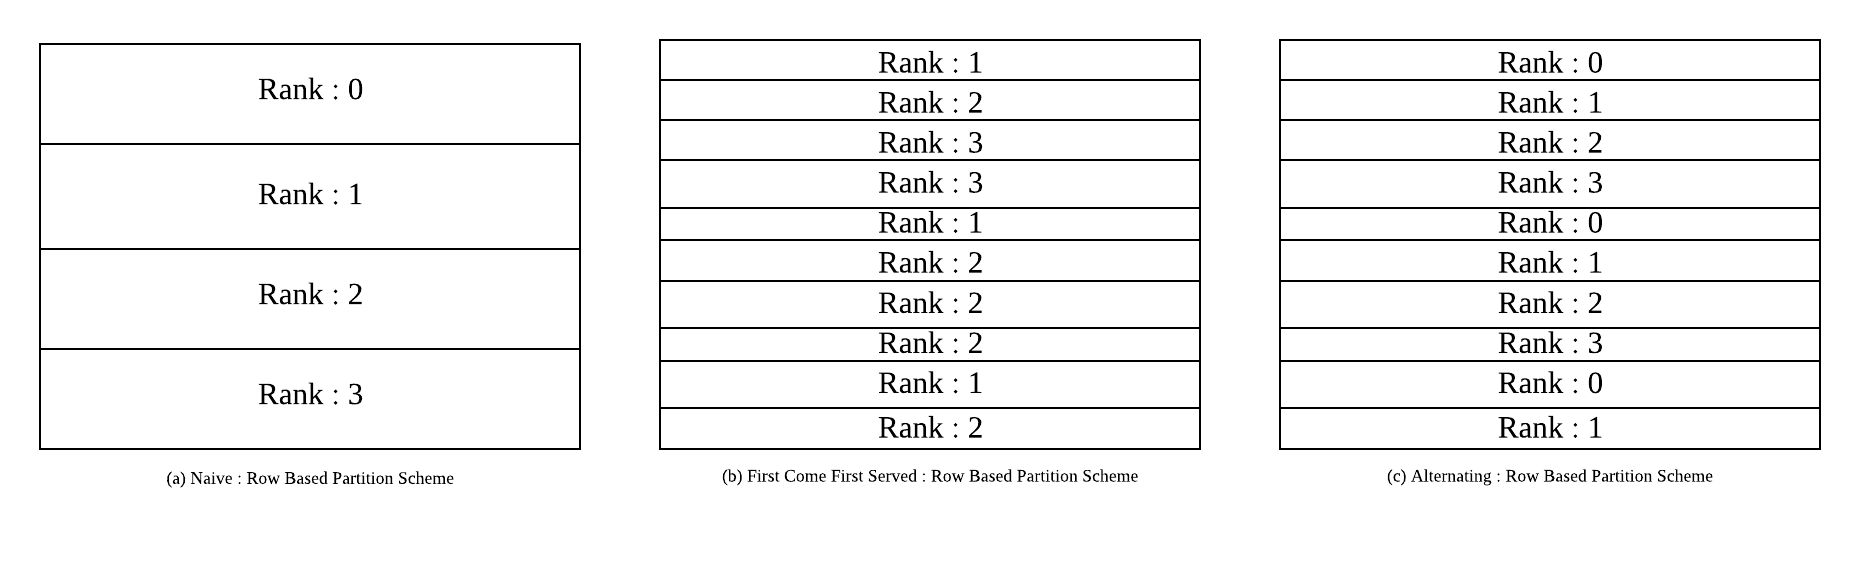
\includegraphics[width=3.4in]{P_SCHEME}  \label{Partition}
			\caption{Partition Schemes when $N=4$ }
		\end{figure}
			\subsection{Naive : Row Based Partition Scheme }\label{Naive}
			As shown in <enter>, the final image is divided equally among N number of processors. So each process will pre-calculate its start and end positions and generate the Mandelbrot Set for that portion. The equation used to calculate the start ($S_r$) and end point ($E_r$)  for each processor with rank ($r$) is shown below.
			
			\begin{equation}
			S_r = \frac{iYmax}{\text{number of tasks}} \times \text{rank}
			\end{equation}
			
			\begin{equation}
			E_r = iYmax {  } \%  {  }  \text{number of tasks}
			\end{equation}
			
			Using this partition scheme each process get an equal amount of rows to work with, which can be written using the following equation.
			\begin{equation}
				\label{rowsPerTask}
				\text{rows per task} = \frac{iYmax}{\text{numer of tasks}}
			\end{equation}
			
			In the case where the number of rows cannot be equally divided among the number of tasks, the last node (rank = $N$ - 1) will calculate the remaining set of rows. \newline
			After generating the $S_r$ and $E_r$ points,  all of the nodes will generate the $Cy$ and $Cx$ arrays. Then the master node will open the file and it will start generating the Mandelbrot Set for the rows allocated for it. The other nodes will also use the $S_r$ and $E_r$ points to generate their specific rows. Finally, all the slave nodes will send their generated values to the master node. The master node will then receive the chunks of rows and write it to the file. The technical flowchart for the Naïve row based partition scheme is shown in Figure \ref{Naive_1}.
			
			\begin{figure}[h]
			\centering
			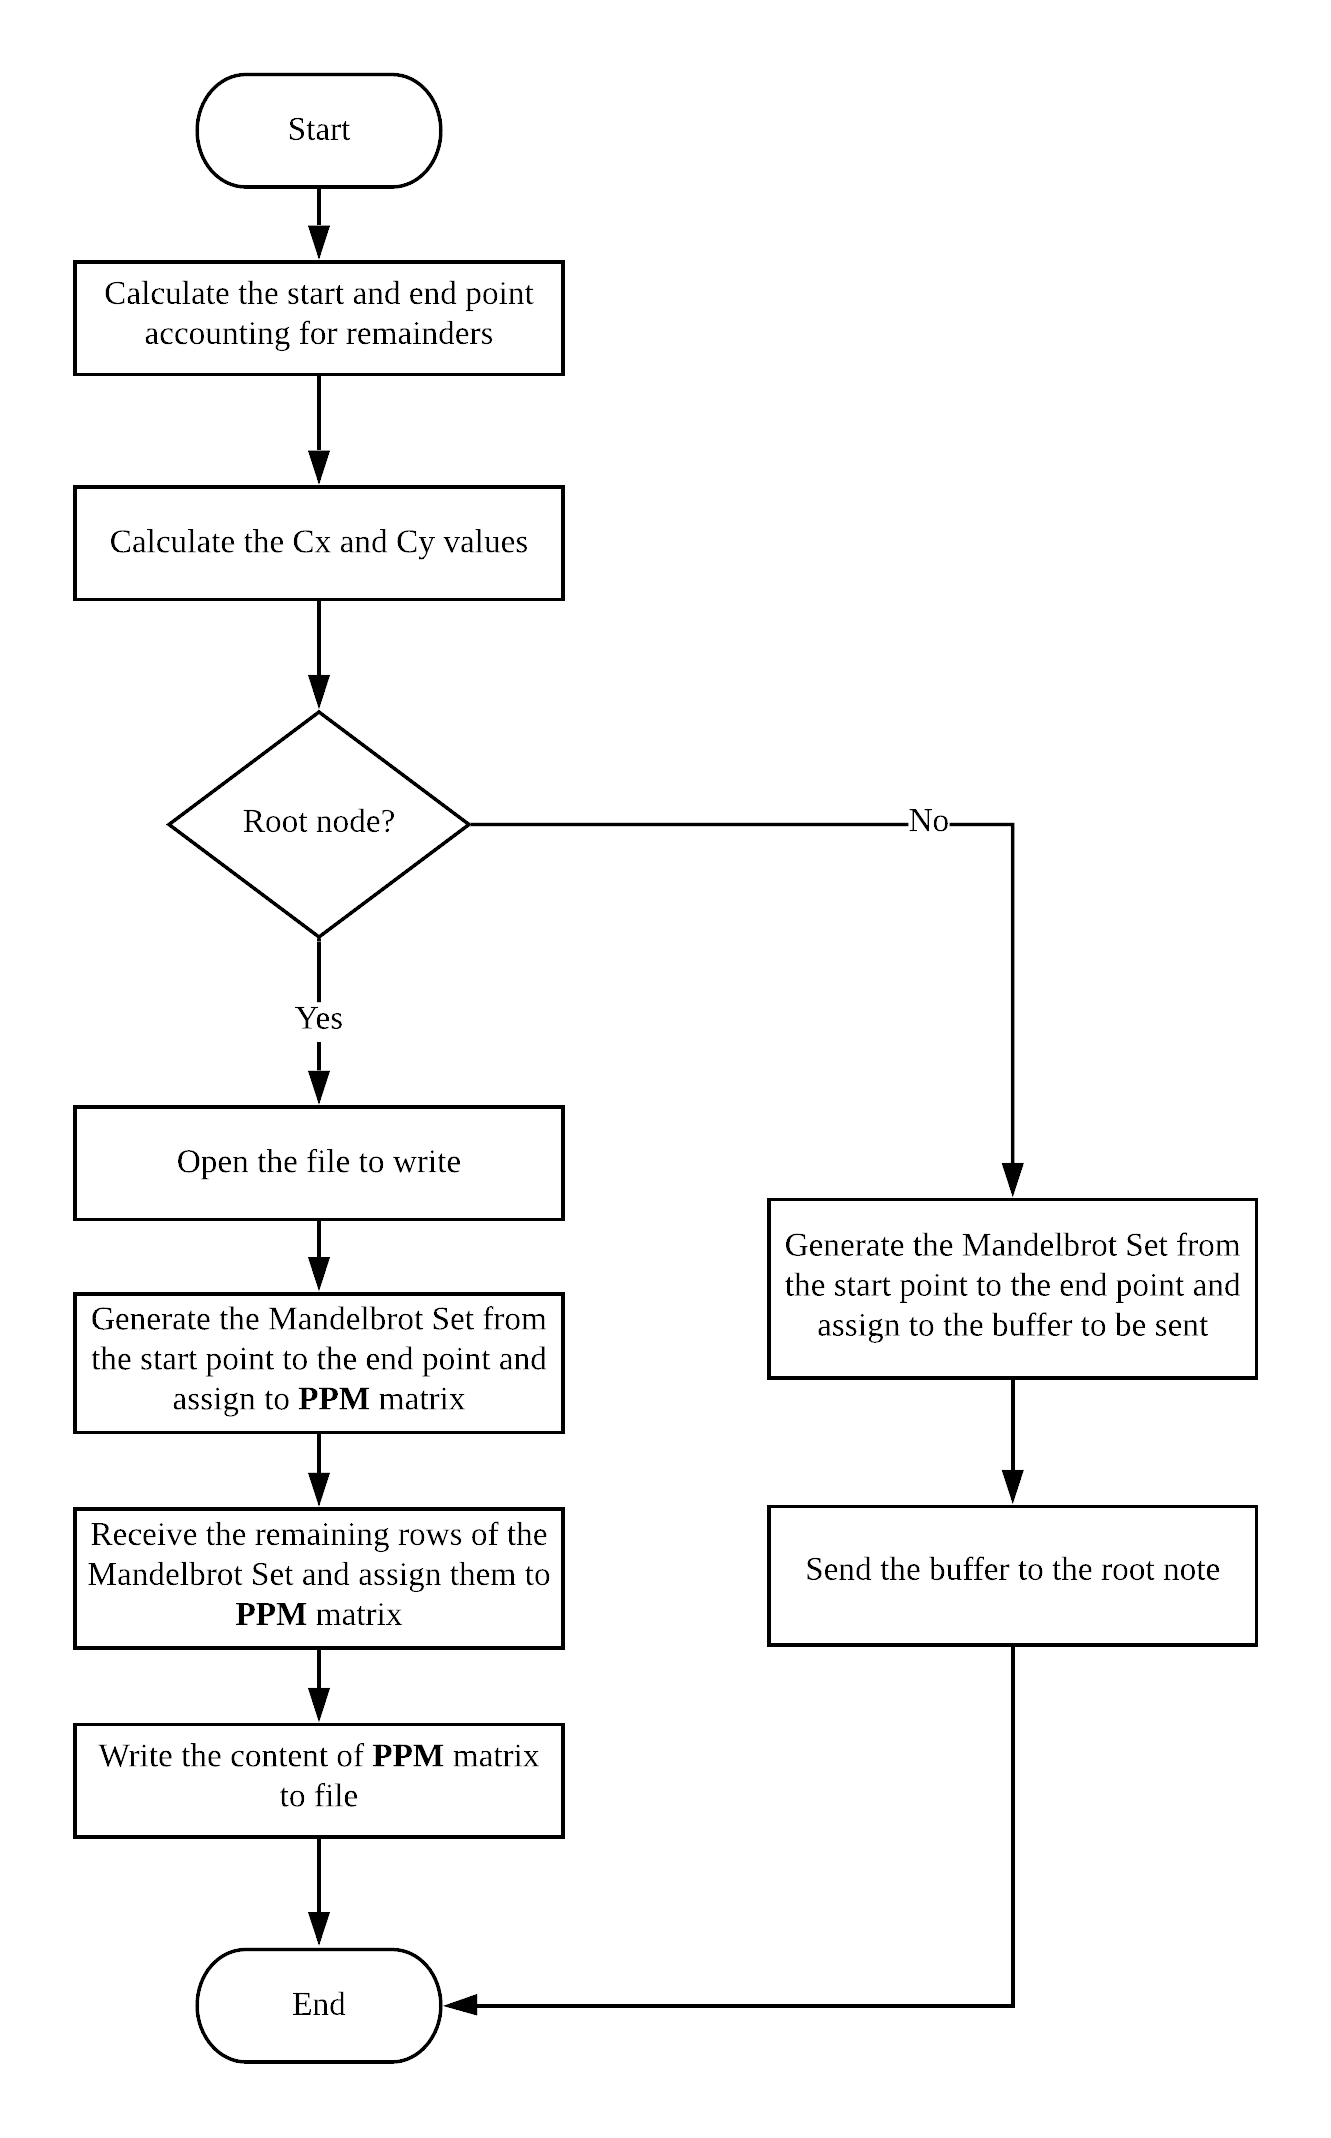
\includegraphics[width=3in]{Naive}
			\caption{Technical Flowchart for Naïve Row Based Partition Scheme}
			\label{Naive_1}
			\end{figure}
			
			
			\subsection{First Come First Served : Row Based Partition Scheme}\label{FCFS}
			This partition scheme shares similarity with Schedulers, where the master node sends work based on the availability.As shown in Fig  <enter> the order in, which node performs which row is based on the availability of the node. If one node finishes the work allocated to it, then it will proceed to the next row. So the master node keeps track of the rows that are processed so far and it will send the next row to the next available task. The slave node will then receive the row number and calculate the Mandelbrot set for that row. This will be done until the master node sends a row number larger than $iYmax$. At that point the node has finished all of the work so it will stop and exit the program. The master node will copy each row received from the slaves and use the row number to decide which row it is, and add it to the memory. Then after receiving all the rows, it will write the data from memory to file. For this partition scheme, the issue of having an odd core count or row values is not present since its based on the availability. 
			Due to the nature of work allocation, this partition scheme is named as First Come First Served. The main this to note is that the master node does not perform in generation. It will only be delegating work to the slave nodes. The technical flowchart for the First Come First Served row based partition scheme is shown in Figure \ref{FCFS_i}.
			
			\begin{figure}[h]
				\centering
				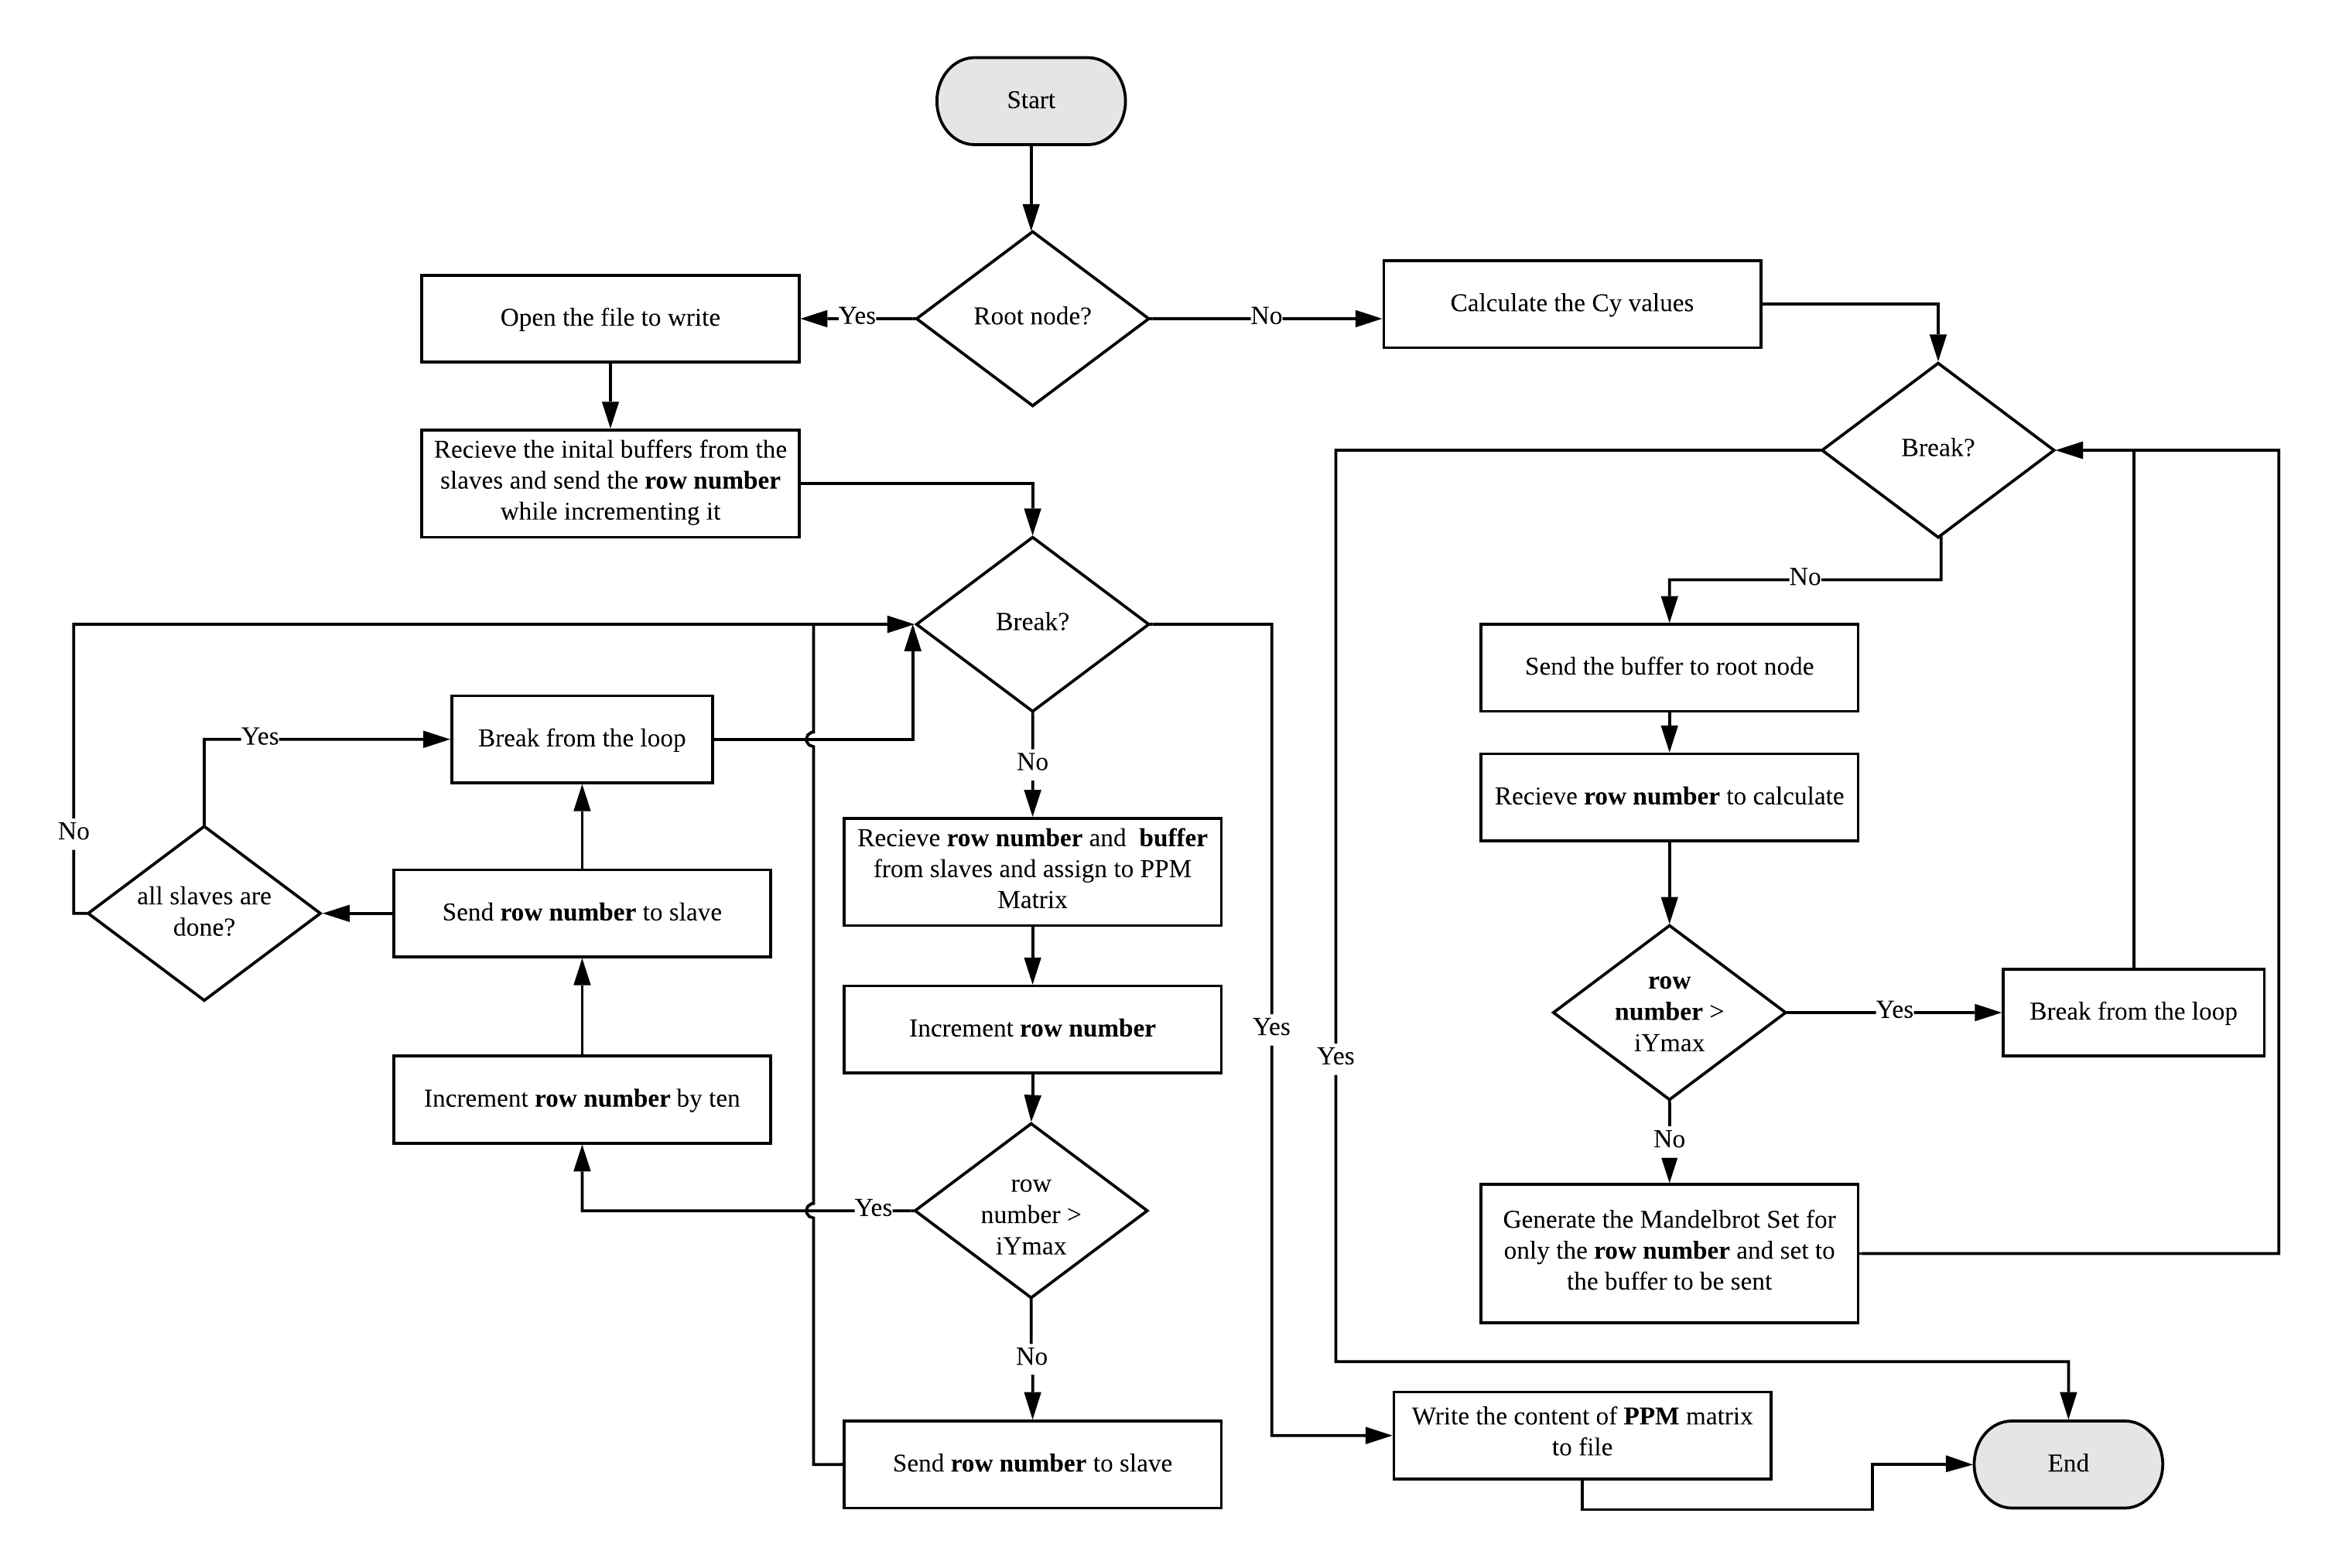
\includegraphics[width=3in]{FCFS}
				\caption{Technical Flowchart for First Come First Served Row Based Partition Scheme}
				\label{FCFS_i}
			\end{figure}
	
			\subsection{Alternating : Row Based Partition Scheme}\label{Alternating}
			This partition scheme is similar to \ref{Naive}, where all the tasks divide the work among themselves initially.Figure <> shows that each task will perform the alternating rows, thus dividing the number of rows equally. In the case where the number of rows cannot be equally divided, the master node will then perform the remainder. Initially all the nodes calculate the $Cy$ and $Cx$ values. The master node then opens the file and start calculating the rows starting from the $0^{th}$ index until the end, with increments of the number of tasks. Similarly, each node starts from their respective rank and increment with the number of tasks. Similar to \ref{Naive}, each process get an equal amount of rows to work with, which can be written using equation \ref{rowsPerTask}. Then all the slave nodes sends back the generated rows to the master node. Before receiving, if there is a remainder, the master node will increment one by one to calculate it. After receiving all the rows, the master node will loop though the $0^{th}$ index till $iYmax$ and reconstruct the image collecting alternate rows from the received arrays. Then it will write all the data into the file.
			The technical flowchart for the Alternative row based partition scheme is shown in Figure \ref{Alte}.

			\begin{figure}[H]
				\centering
				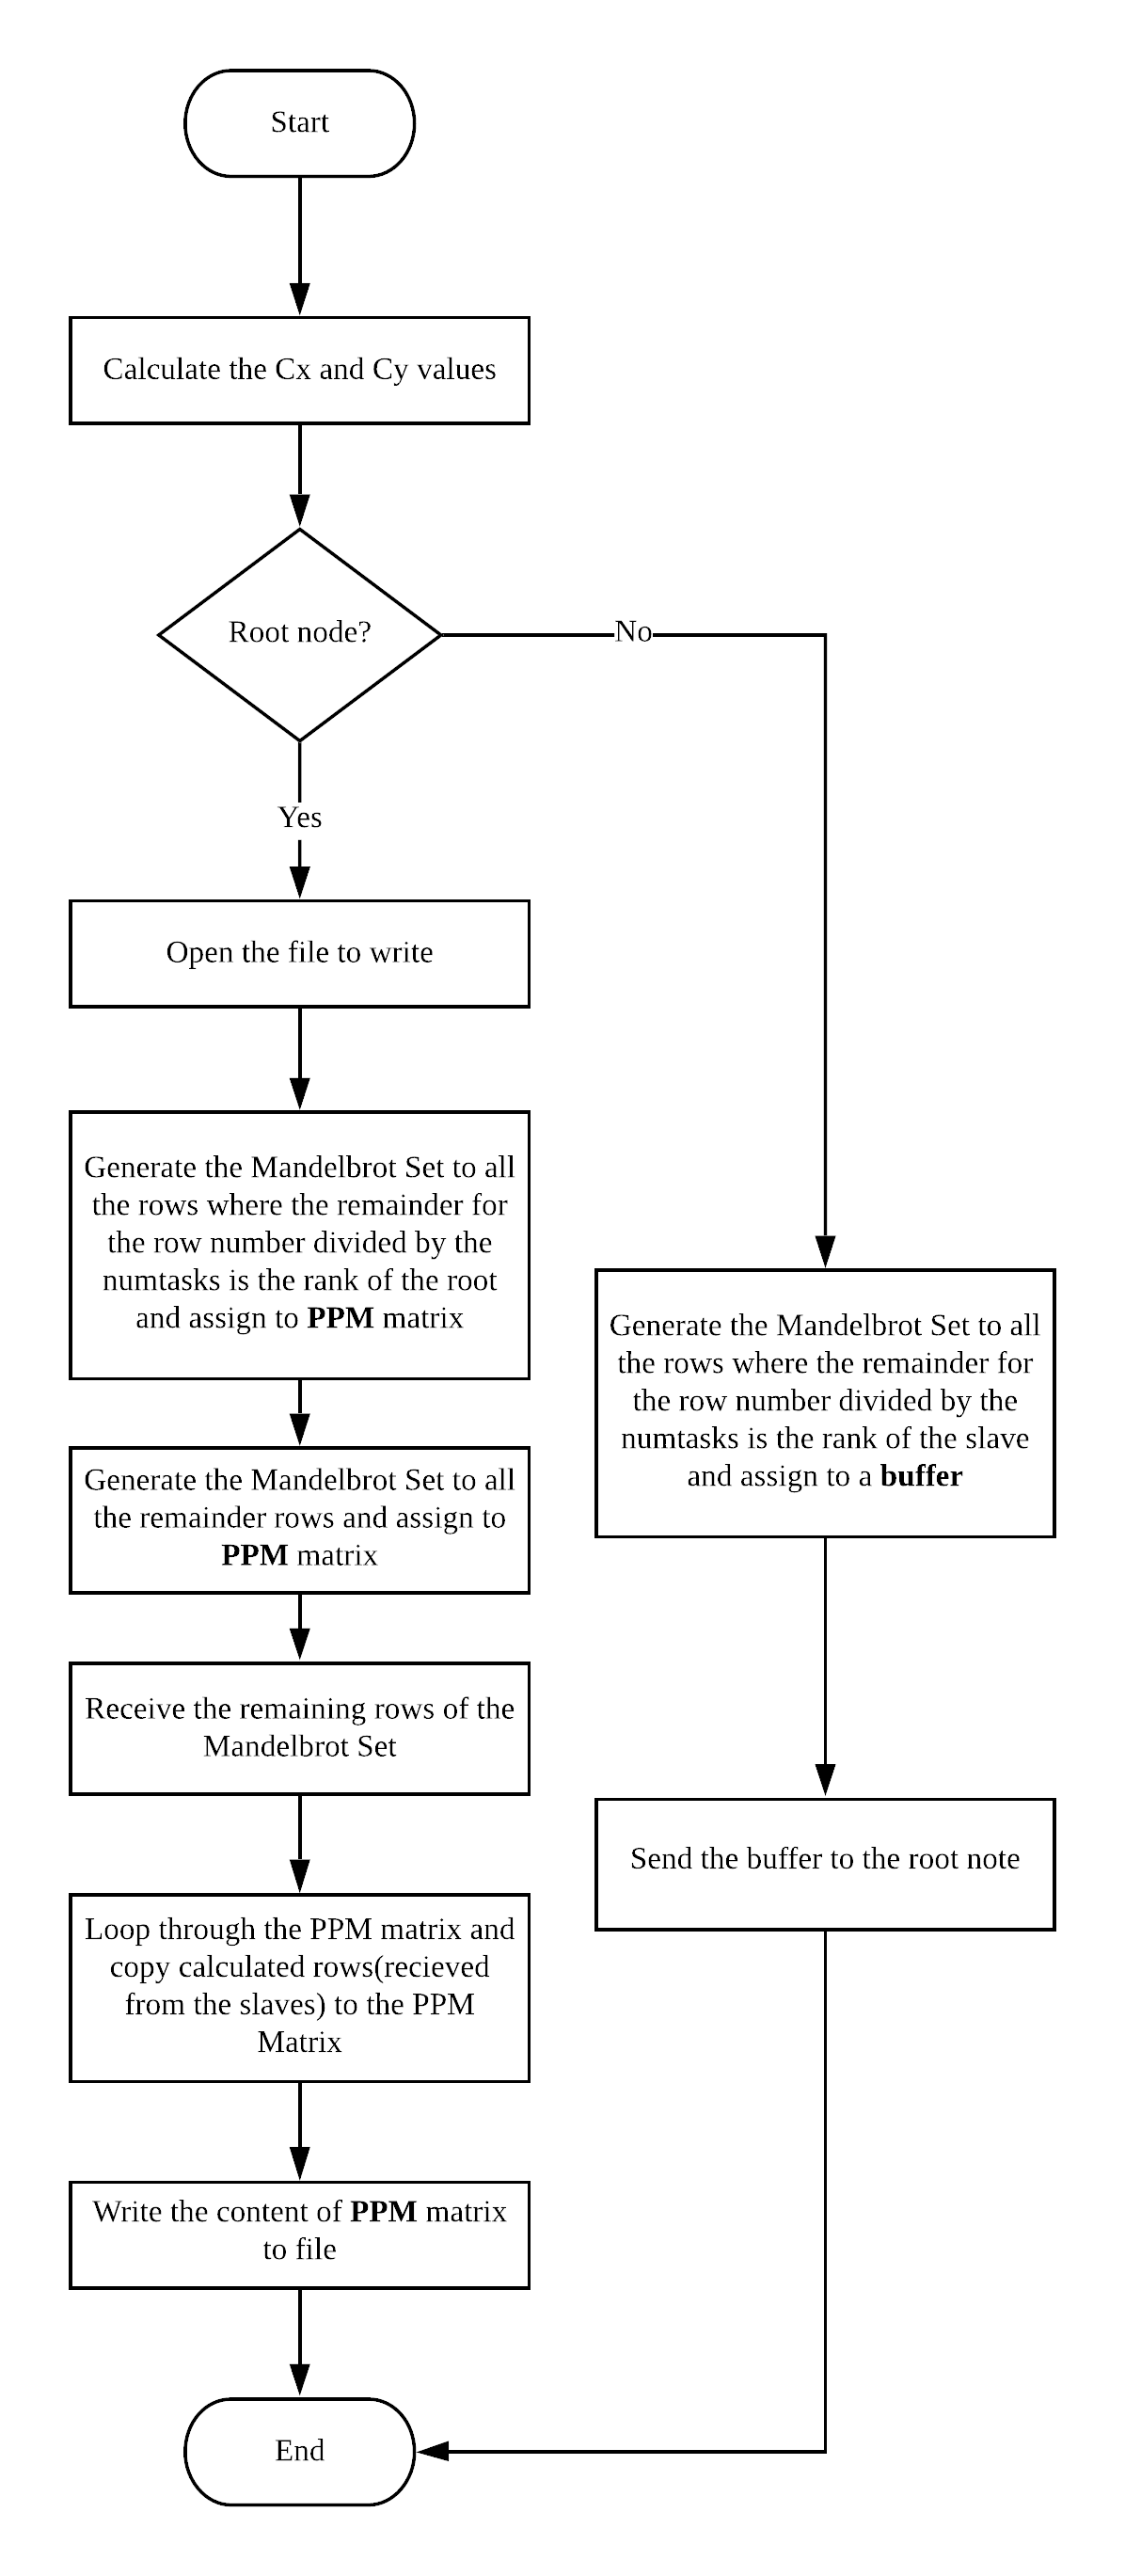
\includegraphics[width=3in,height=6in]{Alternating}
				\caption{Technical Flowchart for Alternative Row Based Partition Scheme}
				\label{Alte}
			\end{figure}

\begin{table*}
	\centering
	\caption{Analysis of Theoretical Speedup vs Actual Speedup}
	\subfloat[Theoretical Speedup vs Actual Speedup of all the partition schemes]
	{
		\renewcommand{\arraystretch}{1.2}
		\label{ac}
		\begin{tabular}{|p{0.5cm} |p{1.5cm}|p{1.5cm}|p{1.5cm}|p{1.5cm}|}			
			\hline
			\textbf{N} & \multicolumn{1}{p{1.5cm}|}{\textbf{Theoretical Speedup}} & \multicolumn{1}{p{1.5cm}|}{\textbf{Naïve Row-Based}} & \multicolumn{1}{p{1.5cm}|}{\textbf{First Come First Served}} & \multicolumn{1}{p{1.5cm}|}{\textbf{Alternating Row-Based}} \\ \hline
			2  &   1.99440	&1.97812&	1.00396	&1.99000  \\ \hline
			4  &   3.96659	&2.05984	&2.98414	&3.96060  \\ \hline
			8  &    7.84583	&2.49809	&6.77486	&7.60671    \\ \hline
			16 &   15.35350	&3.97305	&13.33375	&13.37449  \\ \hline
			32 &   29.43820	&7.37966	&23.72932	&22.87749 \\ \hline
			$\infty$ &      356.22764   &  - &  - &    -  \\ \hline
			
		\end{tabular}
	}
	\subfloat[Percentage Difference of all the partition schemes]
	{
		\renewcommand{\arraystretch}{1.2}
		\label{pd}
		\begin{tabular}{|p{0.5cm}|p{1.5cm}|p{1.5cm}|p{1.5cm}|}			
			\hline
			\textbf{N} & \multicolumn{1}{p{2cm}|}{\textbf{Naïve Row-Based}} & \multicolumn{1}{p{2cm}|}{\textbf{First Come First Served}} & \multicolumn{1}{p{2cm}|}{\textbf{Alternating Row-Based}} \\ \hline
			2  &   0.81952&	66.06515&	0.22072  \\ \hline
			4  &  63.27981&	28.26920&	0.15114  \\ \hline
			8  &   103.39878&	14.65004&	3.09480   \\ \hline
			16 &  117.77011&	14.08118&	13.77758 \\ \hline
			32 &  119.82522	&21.47507&	25.08121 \\ \hline
			$\infty$ &   - &  - &    -  \\ \hline
			
		\end{tabular}
}
\end{table*}

	\section{Test Methodology}
	 \label{TEST}
	In order to calculate the run times for the three partition schemes multiple tests were done. For each tests we set the size of the image to 8000 $\times$ 8000 with 2000 iterations. An assumption taken for the test cases was that the core count will always be a multiple of 2, but all of these partition schemes will work with any other core count, as all of them have a method to handle remainders. Each partition scheme was executed 5 times, with 2, 4, 8, 16 and 32 cores. \newline
	All of the tests were done on the MonARCH (Monash Advanced Research Computing Hybrid) HPC/HTC cluster. The problem with using a cluster is that the scheduler decide which CPU to use based on some predefined rules such as availability. So for our tests to be equal, a constraint was added in order to limit the tests to only one CPU type. All the tests were done on Intel® Xeon® Gold 6150 Processors with 36 logical cores. But since hyper threading was turned off, each processor had only 18 cores. So in order to run the 32 task process, two 16 core processors were used. Listing 2 of the appendix, shows the job file used to run the parallel code with 32 cores. The RAM was set to 32GB for all the tests. \newline
	For each test, we calculated the time taken for generating the Mandelbrot Set and also the total time taken including the writing of data to the file. All the results and the server output files are attached in the appendix. 
	
	When generating the Mandelbrot Set, the main property to note is the time taken to process each section of the image. The top and bottom parts of the image takes less time compared to the middle portion of the image. So each of the partition schemes will require to balance the work load not only by the amount of rows, but also based on the partition scheme that makes use of all the tasks equally.

	\begin{figure*}[!t]
		\centering
		\caption{Plots for Theoretical Speedup vs Actual Speedup}
		\subfloat[Theoretical Speedup vs Actual Speedup]
		{
			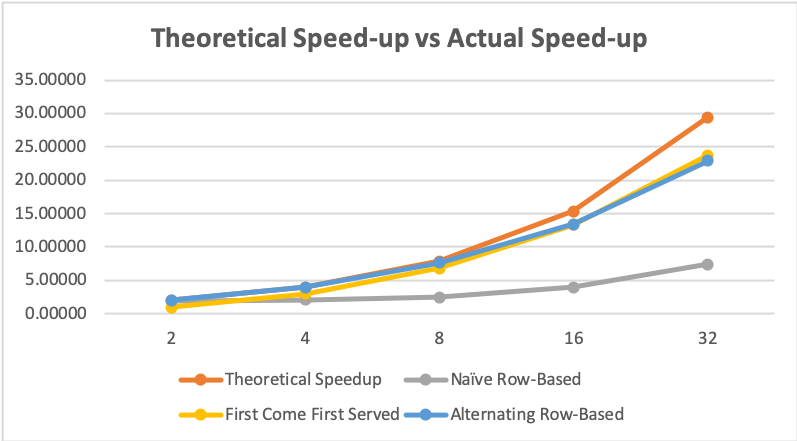
\includegraphics[width=3in]{theo1}
			
		}
		\subfloat[Percentage Difference]
		{
		
			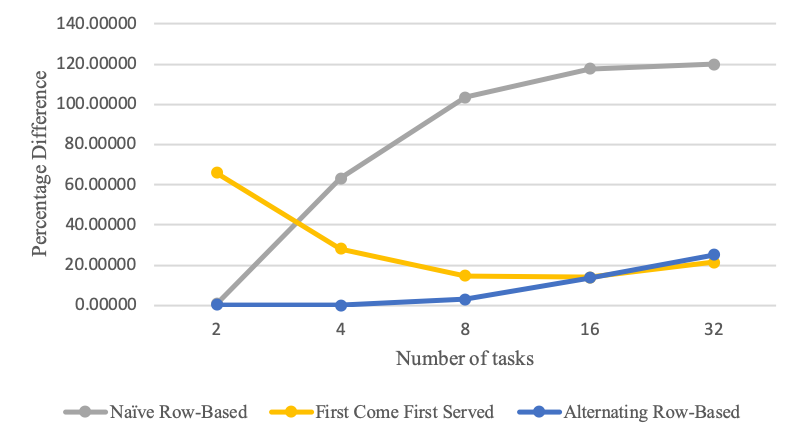
\includegraphics[width=3in]{theo2}
			\label{dpd}
		}
	\end{figure*}
	\section{Results and Discussions}
	
	
	Now let us discuss about the results obtained from the testing phase. Each partition scheme will be compared and discussed based on the following criteria. 
	
	\begin{itemize}
		\item Theoretical Speed-up vs Actual Speed-up
		\item Actual Speed-up between each partition scheme
	\end{itemize}

	\subsection{Theoretical Speed-up vs Actual Speed-up}
	
	In this section we will compare how the actual speed up compared against the theoretical speed up established in Section \ref{Theo}
	
	\subsubsection{Naive - Row Based Partition Scheme }
	\label{naiveres}
	This method divides the whole image into $N$ number of parts, where $N$ is the number of tasks.
	Referring to Table \ref{ac}, for 2 cores, the theoretical speed and the actual speed-up if almost equal. The main reason for this is when we are using two cores, the workload is divided equally among the two processes. Both the tasks will be doing the high iteration and low iteration part of the image.
	But when the number of cores increase, the actual speed up becomes poor. The reason for this, even though the tasks get equal rows, is the number of iterations needed for some rows are greater than others, as mentioned previously in Section \ref{TEST}. Due to this, the tasks in-charge of the top and bottom quarter of the image takes less time compared to the middle part, so the master node has to wait until all the tasks are complete to write the file. Finally comparing the percentage difference \ref{pd} we see that this partition scheme does not perform well when the core count increases.
	
	\subsubsection{First Come First Served - Row Based Partition Scheme}
	This method sends the row based on the availability of the task. Looking back at Table \ref{ac}, we see that the performance of the 2 core is almost equal to no speed up at all. The main reason for this is when we use a two core the slave generates all the rows in the image, while the master sends and receives data. So the actual speedup should be $ \le 1$, but our actual speedup $> 1$. Why?. According to a paper published in 2016, by a group of researchers \cite{ristov2016superlinear}, this behavior is common in parallel systems as the serial program needs more RAM to store the data while generating the image, the parallelized system can use the cache as it can store the small chunks of data received at each send and receive. Therefore the speedup can be $\ge 1$ even with a lot of communication.	
	Next, comparing the theoretical speed up vs actual speed up for multiple cores, we see that this partition scheme is sub-linear. The percentage difference is at a reasonable difference, but when two cores are used, it does not perform well because of the reasons mentioned above. But the percentage difference decreases with each increment of the core count.
	
	\subsubsection{Alternating - Row Based Partition Scheme}
	This method divides the rows based on the rank number of each task. Referring to Table \ref{ac}, this approach is almost equal to the theoretical speedup when two cores are used. The reason is the same as \ref{naiveres}, where the work load is divided equally among the two tasks. Even when the number of cores increases, this method is able to perform in a sub-linear order staying close to the theoretical limit. Referring at Table \ref{pd}, we see that the the percentage difference increases with each increment in the number of cores.
	
	Now that we have an idea about the difference between the Theoretical Speed-up and Actual Speed-up , let us look into how they compare up against each other.
	
	\subsection{Actual Speed-up between each partition scheme}
	
		\subsubsection{Naïve - Row Based Partition Scheme }
		Comparing the Naïve approach with the rest, we immediately notice the performance is poor. But evaluating dual core performance, this approach performs better than the First Come First Served approach. But as the core count increases, this approach cannot keep up with the other two partition schemes. Therefore we can conclude that this partition scheme performs the worst out of the three approaches.
	\subsubsection{First Come First Served - Row Based Partition Scheme}
	\label{fcfsex}
		Comparing this approach with the rest, we see that it performs average, but as the core counts increases, we see that this performs better than any of the other methods. The reason for this is, both the other methods cause a bottle neck when they send the data at the same time to the master. If the work load is divided equally, then all the slaves finishes at the same time thus causing a bottle neck at the master node. 
		
		But First Come First Served approach uses more communication to ensure that the bottle neck is amortized over all the communication instead of all at once. So the master node does not have to copy all the rows from each task at the end. It will do it as the tasks finish each row. This leads to the First Come First Served partition approach to be faster when the core count is higher.
	
	\subsubsection{Alternating - Row Based Partition Scheme}
	
	Comparing this approach with the Naïve approach, for two cores we see that the work load distribution is the same. But why is it faster compared to Naïve approach?. The reason is the master node is computing the high iteration part at the end, so even though the slave finishes at the same time, it has to wait till the master node is ready to receive.In the alternating approach, each process get the high iterating part at middle, so they finish at the same time, thus reducing the wait time for the slave.
	
	Referring to Figure \ref{dpd}, we see that the First Come First Served approach, is faster than the Alternating approach when the number of tasks is increased. The reason of this is explained in \ref{fcfsex}.

	\section{Conclusion}
	Now that we have considered all the cases
	

	\section{Future Work}
	
	

	
\bibliographystyle{IEEEtran}
\bibliography{ref.bib}

	\newpage
	\onecolumn
	\appendix
		\begin{figure*}[h]
		\centering
		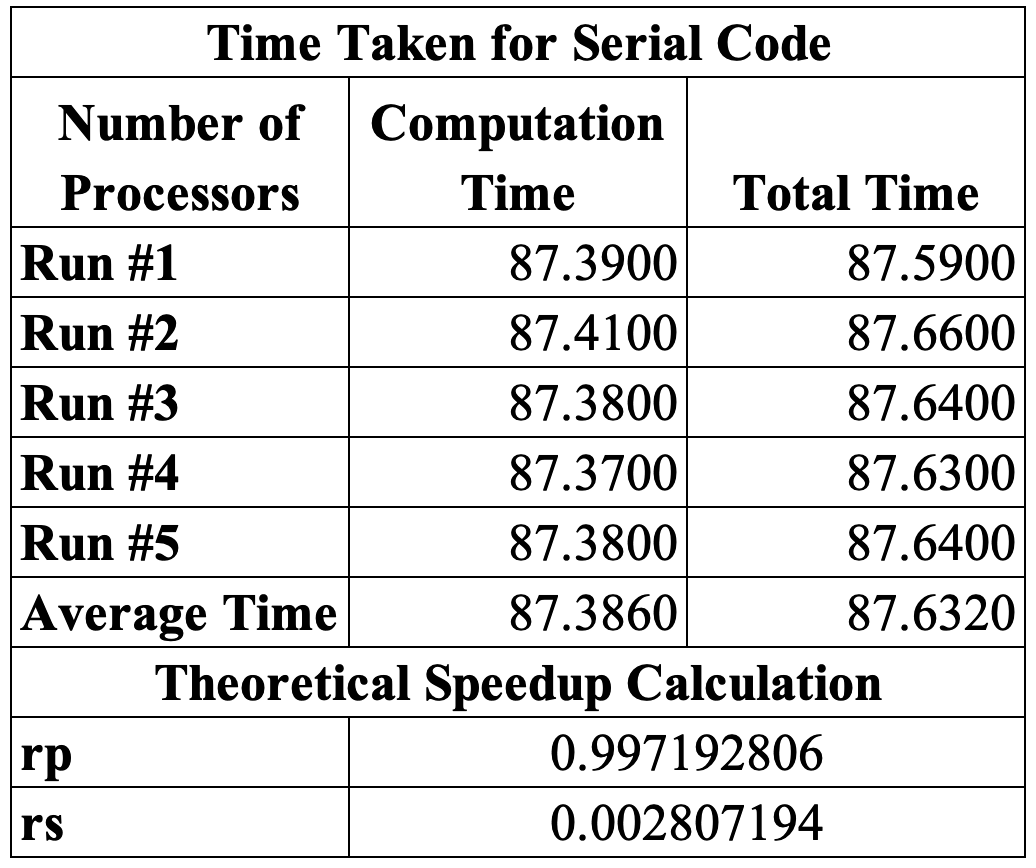
\includegraphics[width=7cm,keepaspectratio]{SCal}
		\caption{Property profile of the diverse library compared to the compound pool.}
		\label{fig:PropProf}
	\end{figure*}
	\newpage
	\begin{sidewaysfigure*}[h]
		\centering
		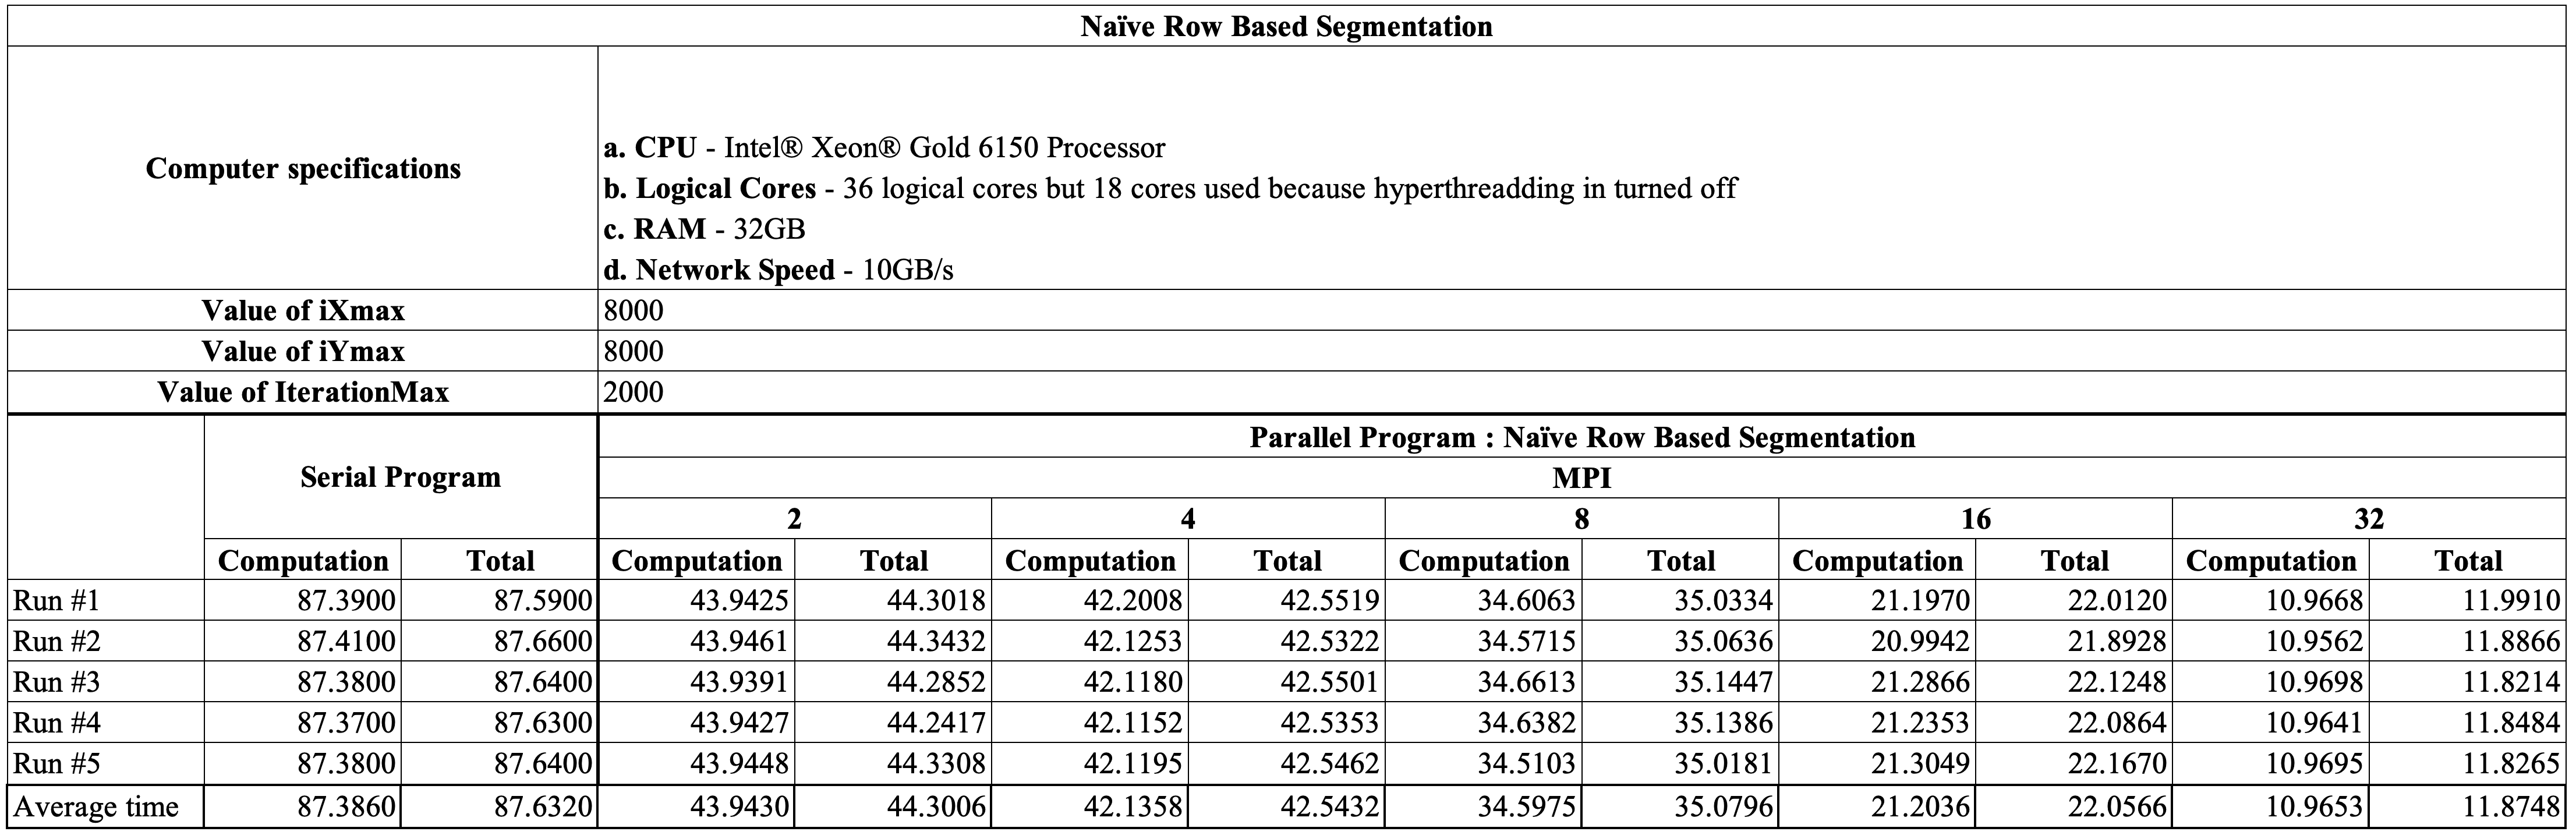
\includegraphics[width=\textheight,height=\textwidth,keepaspectratio]{NaiveCal}
		\caption{Test Results : Naïve Row Based Segmentation}
		\label{fig:PropProf}
	\end{sidewaysfigure*}
\newpage
	\begin{sidewaysfigure*}[ht]
	\centering
	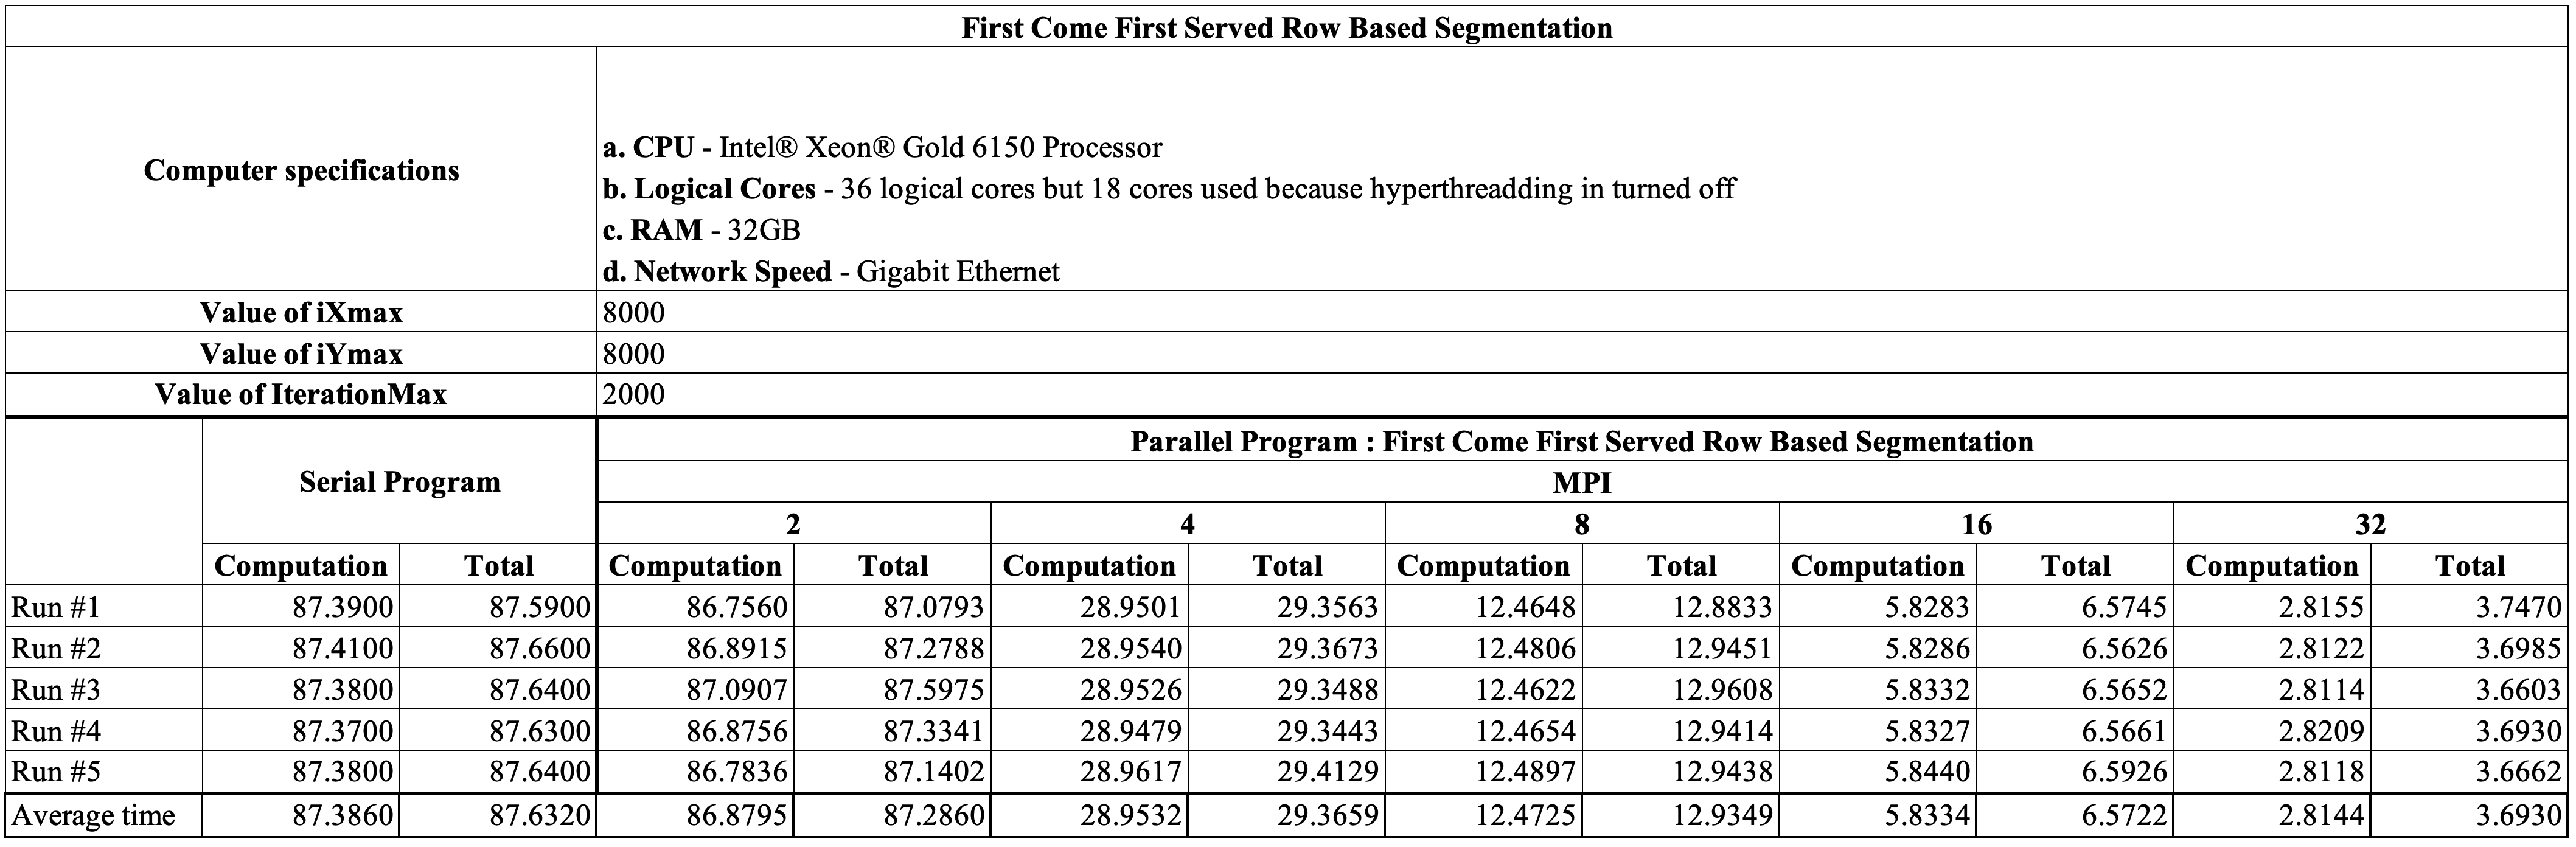
\includegraphics[width=\textheight,height=\textwidth,keepaspectratio]{FCFSCal}
	\caption{Test Results : First Come First Served Row Based Segmentation}
	\label{fig:PropProf}
\end{sidewaysfigure*}
\newpage
	\begin{sidewaysfigure*}[ht]
	\centering
	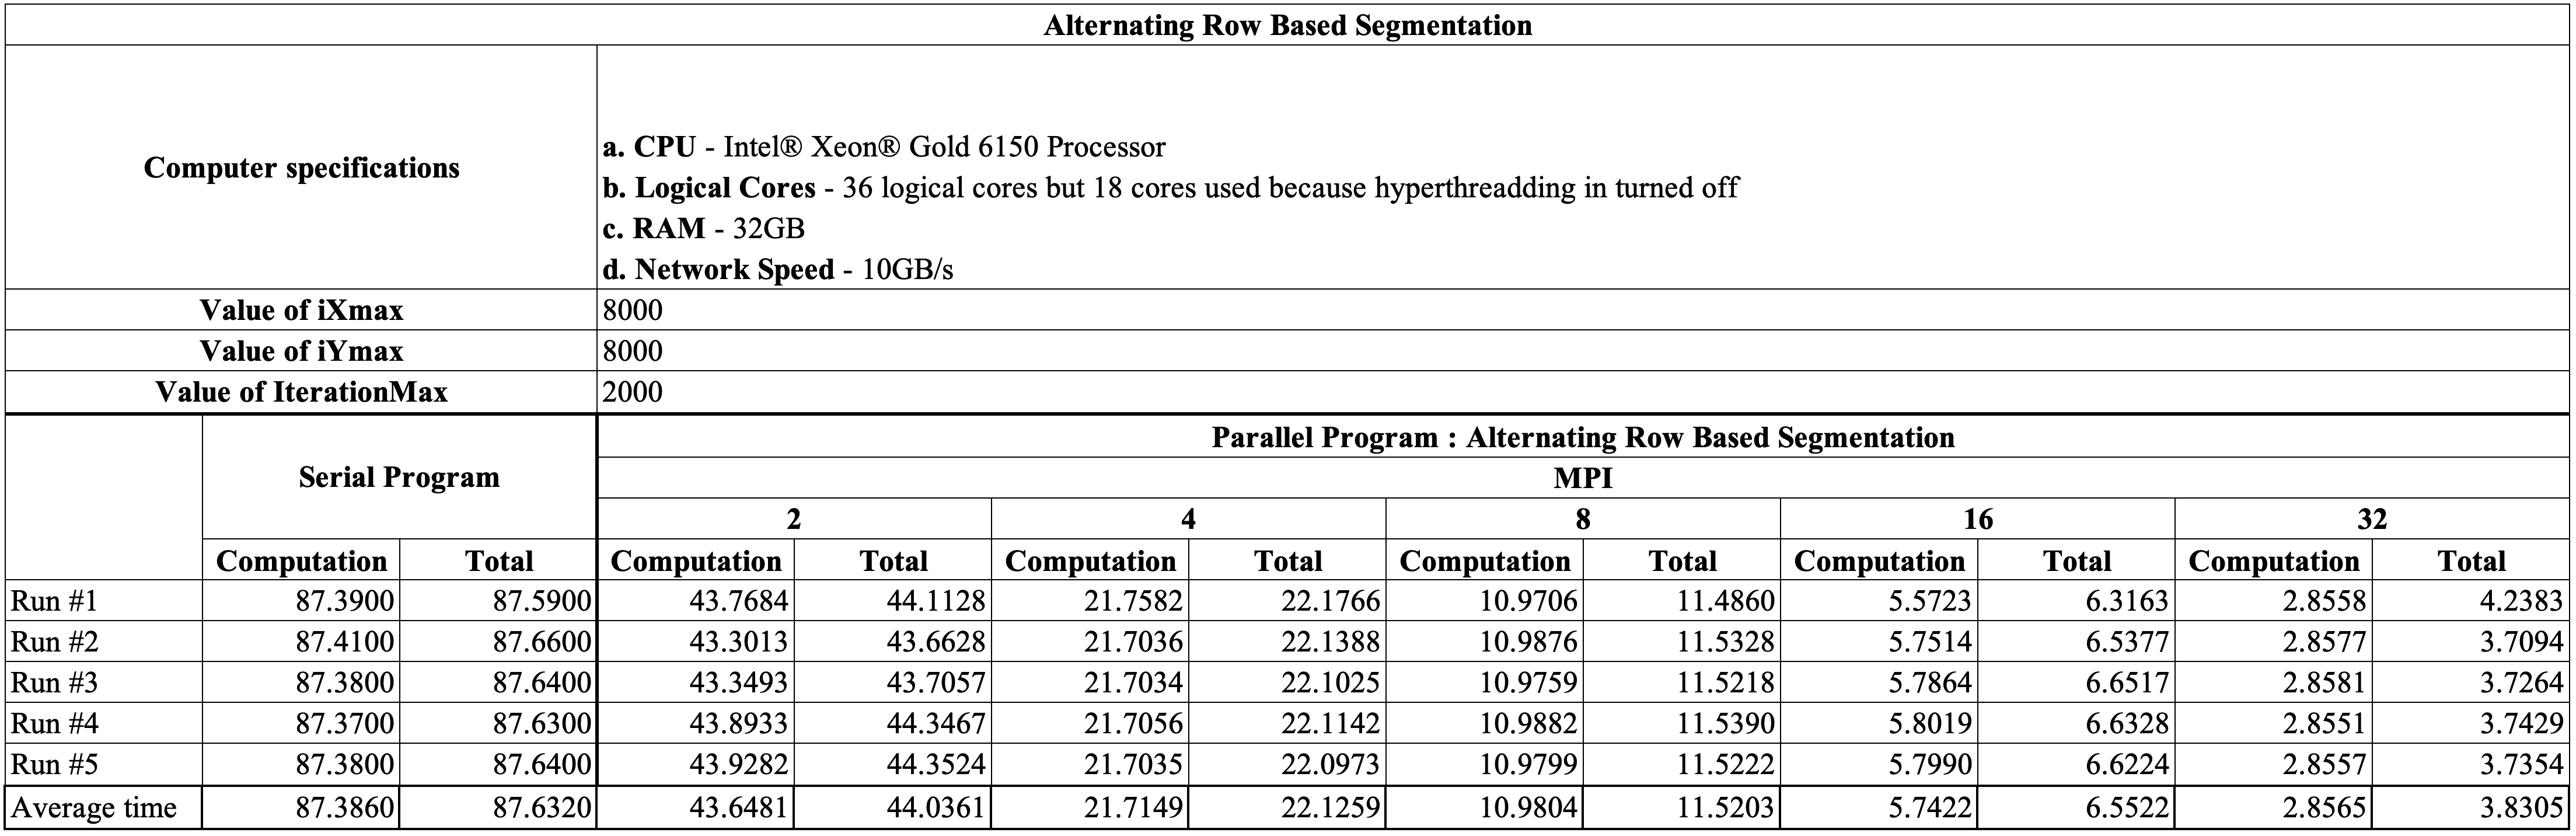
\includegraphics[width=\textheight,height=\textwidth,keepaspectratio]{AlCal}
	\caption{Test Results : Alternating Row Based Segmentation.}
	\label{fig:PropProf}
\end{sidewaysfigure*}
\newpage


\begin{lstlisting}[caption={MonARCH job script for 16 cores},label={16job}]
#!/bin/bash
#SBATCH --job-name=alter_16
#SBATCH --time=00:30:00
#SBATCH --mem=32G
#SBATCH --ntasks=16
#SBATCH --cpus-per-task=1
#SBATCH --ntasks-per-node=16
#SBATCH --account=fit3143
#SBATCH --constraint=Xeon-Gold-6150
#SBATCH --output=alter_16.out
module load openmpi/1.10.7-mlx

echo "Alternative : 16 cores"

echo "Run 1"
srun mandelbrot_parallel_alternating

echo "Run 2"
srun mandelbrot_parallel_alternating

echo "Run 3"
srun mandelbrot_parallel_alternating

echo "Run 4"
srun mandelbrot_parallel_alternating

echo "Run 5"
srun mandelbrot_parallel_alternating

\end{lstlisting}

\begin{lstlisting}[caption={MonARCH job script for 32 cores},label={32job}]
#!/bin/bash
#!/bin/bash
#SBATCH --job-name=alter_32
#SBATCH --time=00:30:00
#SBATCH --mem=32G
#SBATCH --ntasks=32
#SBATCH --cpus-per-task=2
#SBATCH --ntasks-per-node=16
#SBATCH --account=fit3143
#SBATCH --constraint=Xeon-Gold-6150
#SBATCH --output=alter_32.out
module load openmpi/1.10.7-mlx

echo "Alternative : 32 cores"

echo "Run 1"
srun mandelbrot_parallel_alternating

echo "Run 2"
srun mandelbrot_parallel_alternating

echo "Run 3"
srun mandelbrot_parallel_alternating

echo "Run 4"
srun mandelbrot_parallel_alternating

echo "Run 5"
srun mandelbrot_parallel_alternating



\end{lstlisting}

\end{document}
